% questions.tex —— 1980 年·全国卷（文科） · 题目内容片段（无答案）
% 由 tools/generate_projects.py 依来源总账自 1980/1980_数学真题_文_试题.md 生成，勿手改（改源 MD 后重跑）


\begin{gktip}
\textbf{来源说明}：本卷为 1980 年全国统一命题的\textbf{文科数学}卷（同年另有独立的理科卷，两份试卷题目不同），单页（原卷页码第 16 页），全卷共 8 题。题面不含答案（答案由本库独立推导）。

\textbf{题面说明}：第 7 题依原卷配图重绘为 TikZ 矢量图（长方体 $ABCD\text{-}A'B'C'D'$）。原卷第 7 题“$AE$ 与底面的对角线 $B'D'$ 垂直于 $E$”一句，按“$AE$ 与底面对角线 $B'D'$ 垂直、垂足为 $E$”理解；本文照原卷字面转录，未径改。
\end{gktip}

\begin{question}
\gkti{1}化简：$\dfrac{1-3\mathrm i}{3-2\mathrm i}$。

\end{question}
\begin{question}
\gkti{2}解方程组：
\nopagebreak[4]
\[
\begin{cases}
2x-3y-z=5,\\
4x+2y+3z=9,\\
3x+2y=-1.
\end{cases}
\]

\end{question}
\begin{question}
\gkti{3}用解析法证明：直径所对的圆周角是直角。

\end{question}
\begin{question}
\gkti{4}某地区 1979 年的轻工业产值占工业总产值的 $20\%$，要使 1980 年的工业总产值比上一年增长 $10\%$，且使 1980 年的轻工业产值占工业总产值的 $24\%$，问 1980 年轻工业产值应比上一年增长百分之几？

\end{question}
\begin{question}
\gkti{5}设 $\dfrac{3\pi}{4}<\theta<\dfrac{5\pi}{4}$，化简：
\nopagebreak[4]
\[
\frac{\sqrt{\cos\frac{\pi}{4}\sin\left(\frac{3\pi}{4}-\theta\right)\left[\sin(\pi-\theta)-\sin\left(\theta-\frac{\pi}{2}\right)\right]}}{\sin\left(\theta+\frac{\pi}{4}\right)}.
\]

\end{question}
\begin{question}
\gkti{6}

（1） 若四边形 $ABCD$ 的对角线 $AC$ 将四边形分成面积相等的两个三角形，证明：直线 $AC$ 必平分对角线 $BD$；

（2） 写出（1）的逆命题，这个逆命题是否正确？为什么？

\Needspace{0.4\textheight}
\end{question}
\begin{question}
\gkti{7}如图，长方形框架 $ABCD\text{-}A'B'C'D'$ 三边 $AB$、$AD$、$AA'$ 的长分别为 $6$、$8$、$3.6$，$AE$ 与底面的对角线 $B'D'$ 垂直于 $E$。

（1） 证明 $A'E\perp B'D'$；

（2） 求 $AE$ 的长。
\nopagebreak[4]
\begin{center}% 1980 年全国卷（文科）第 7 题：长方体 ABCD-A'B'C'D'（AB=6、AD=8、AA'=3.6），底面对角线 B'D' 及 AE、A'E（E 为垂足）；左上、显示 A-A' 等被遮棱为虚线（按源卷布局）
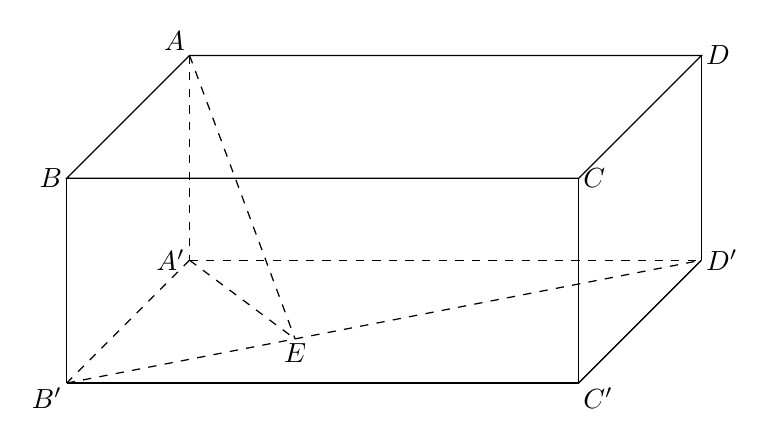
\begin{tikzpicture}[scale=1, line width=0.45pt,
  every node/.style={inner sep=1.5pt}]
  % 顶点（斜二测投影手算：宽 8 单位 -> 6.5cm 水平；深 6 单位 -> 2.2cm 左下 45 度；
  % 高 3.6 单位 -> 2.6cm 竖直）
  \coordinate (A)  at (2.40, 5.80);
  \coordinate (B)  at (0.84, 4.24);
  \coordinate (C)  at (7.34, 4.24);
  \coordinate (D)  at (8.90, 5.80);
  \coordinate (Ap) at (2.40, 3.20);
  \coordinate (Bp) at (0.84, 1.64);
  \coordinate (Cp) at (7.34, 1.64);
  \coordinate (Dp) at (8.90, 3.20);
  % E 为 B'D' 上一点，B'E:B'D' = 3.6:10
  \coordinate (E)  at (3.74, 2.20);
  % 可见棱
  \draw (A) -- (B) -- (C) -- (D) -- cycle;
  \draw (B) -- (Bp);
  \draw (C) -- (Cp);
  \draw (D) -- (Dp);
  \draw (Bp) -- (Cp);
  \draw (Cp) -- (Dp);
  % 不可见棱（虚线）
  \draw[dashed] (A) -- (Ap);
  \draw[dashed] (Ap) -- (Bp);
  \draw[dashed] (Ap) -- (Dp);
  \draw[dashed] (Bp) -- (Dp);
  \draw[dashed] (A) -- (E);
  \draw[dashed] (Ap) -- (E);
  % 顶点标注
  \node[anchor=south east] at (A)  {$A$};
  \node[anchor=east]       at (B)  {$B$};
  \node[anchor=west]       at (C)  {$C$};
  \node[anchor=west]       at (D)  {$D$};
  \node[anchor=east]       at (Ap) {$A'$};
  \node[anchor=north east] at (Bp) {$B'$};
  \node[anchor=north west] at (Cp) {$C'$};
  \node[anchor=west]       at (Dp) {$D'$};
  \node[anchor=north]      at (E)  {$E$};
\end{tikzpicture}
\end{center}
\nopagebreak[4]
\end{question}
\begin{question}
\gkti{8}

\Needspace{5\baselineskip}
（1） 把参数方程
\nopagebreak[4]
\[
\begin{cases}
x=\sec t,\\
y=2\tan t
\end{cases}
\quad(t\ \text{为参数})
\]
化为直角坐标方程，并画出方程的曲线的略图；

（2） 当 $0\le t<\dfrac{\pi}{2}$ 及 $\pi\le t<\dfrac{3\pi}{2}$ 时，各得到曲线的哪一部分？

\end{question}